% ===================================================================================== %
%                                        Header                                         %
% ===================================================================================== %
\documentclass[10pt,t,xcolor=table]{UWMadBeamer}

\usepackage{textcomp}
\usepackage{setspace}
\usepackage{booktabs}
\usepackage{multirow}


\newenvironment{Itemize}
    {\begin{itemize}\setlength{\itemsep}{0.50em}\setlength{\leftmargin}{0.0em}\setlength{\labelwidth}{0em}}
    {\end{itemize}}



\title[MELCOR Analysis of the UW--Madison WRCCS]
    {\texorpdfstring{\underline{\ \ UW--Madison WRCCS\ \ }}{UW-Madison WRCCS} \texorpdfstring{\\[0.25em]}{} MELCOR Analysis of a Scaled NGNP Reactor Cavity Cooling System Experiment}
\institute{MELCOR Cooperative Assessment Program (MCAP)}
\author{%
    \texorpdfstring
        {Troy C. Haskin \\[0.25em]Michael Corradini\\Jae Oh \\Casy Tompkins}
        {Troy C. Haskin, Michael Corradini, Jae Oh, Casy Tompkins}
}
\date[2015-09-17]{September 17, 2015}


\graphicspath{{./Graphics/}}

\setbeamersize{text margin left = 0.03\paperwidth}
\setbeamersize{text margin right = 0.03\paperwidth}

% =========================================================================== %
%                              Document                                       %
% =========================================================================== %
\begin{document}


% ======================================================= %
%                         Titlepage                       %
% ======================================================= %
\begin{frame}
    \frametitle{\ }
    \titlepage
\end{frame}


% ======================================================= %
%                         Outline                         %
% ======================================================= %
\begin{frame}{Outline}
    \tableofcontents
\end{frame}



% ======================================================= %
%                         Motivation                      %
% ======================================================= %
\section{Motivation}

    \begin{frame}
        \frametitle{Reactor Cavity Cooling System (RCCS)}
        \begin{itemize}
            \item Ultimate heat sink for reactor decay heat
            \item Most designed for passive cooling
            \item Two popular fluids: air and water
        \end{itemize}
        
        \begin{table}%
        \caption{List of RCCS designs from \textit{Experimental Studies of NGNP Reactor Cavity Cooling System
With Water} [\href{https://inlportal.inl.gov/portal/server.pt/document/116903/neup_project_no_09-781_final_report_pdf}{\scriptsize pdf}].}
        \vskip-0.8em
        \begin{tabular}{ccccc}
            \toprule
            \textbf{Reactor} & \textbf{Coolant} & \textbf{Mode} & \textbf{Country} & \textbf{Power [MW]} \\
            \midrule
            HTTR & Water & Forced & Japan & 30 \\
            HTR-10 & Water & Natural & China & 10 \\
            PBMR & Water & Natural & South Africa & 265 \\
            GT-MHR & Air & Natural & Russia & 600 \\
            MHTGR & Air & Natural & USA & 450 \\
            \bottomrule
        \end{tabular}
        \end{table}
        
    \end{frame}
    
    \begin{frame}
        \frametitle{PBMR RCCS}
        \begin{figure}%
        \centering
        \caption{From ``PBMR Auxiliary Systems'' [\href{http://pbadupws.nrc.gov/docs/ML0606/ML060680134.pdf}{\scriptsize pdf}], part of \textit{Summary of Public Meeting with PBMR (PTY) LTD} [\href{http://pbadupws.nrc.gov/docs/ML0607/ML060750210.html}{\scriptsize  nrc.gov}].}
        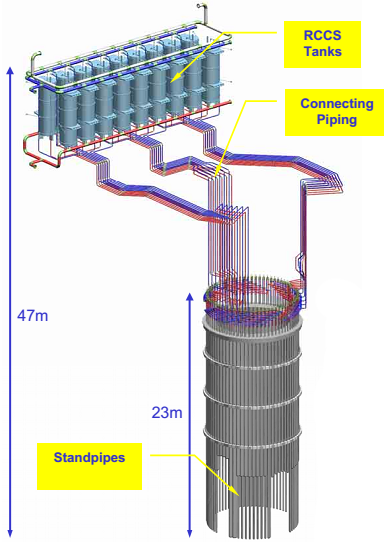
\includegraphics[keepaspectratio,height=0.62\paperheight]{RCCS_PBMR}
        \end{figure}
    \end{frame}


\section{Experiment}

\begin{frame}{WRCCS Purpose}
    \begin{itemize}
        \item Characterize both single and two-phase behavior of a scaled-version of the Reactor Cavity Cooling System (RCCS) with water coolant operating via natural circulation.
    \end{itemize}
\end{frame}

\begin{frame}{WRCCS Facility}
    \begin{columns}
        \begin{column}{0.71\paperwidth}
            \vskip-2em
            \begin{figure}
                \centering
                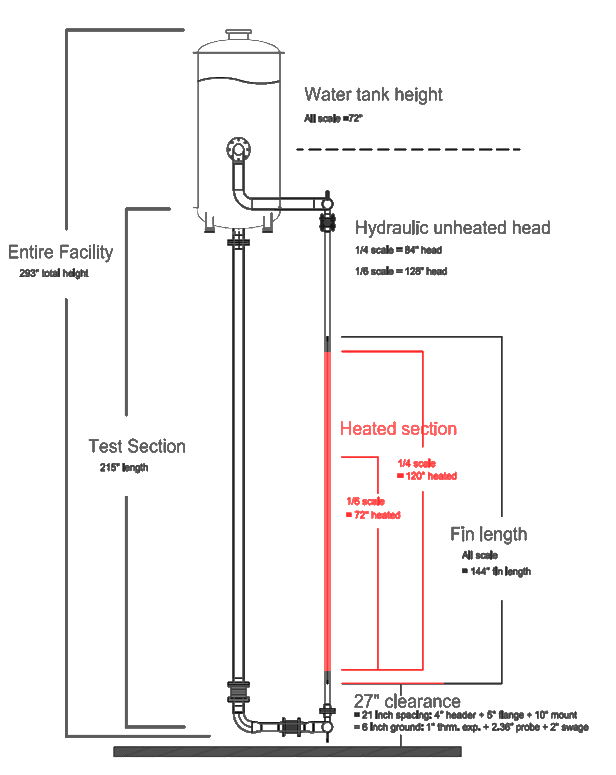
\includegraphics[keepaspectratio,height=0.8\paperheight]{WRCCS_CAD}
            \end{figure}
        \end{column}
        \hfill
        \begin{column}{0.28\paperwidth}
            \begin{figure}
                \centering
                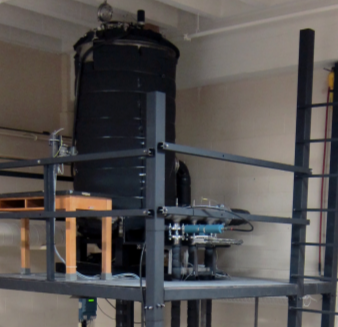
\includegraphics[keepaspectratio,height=0.35\paperheight]{WRCCS_Tank}\\
                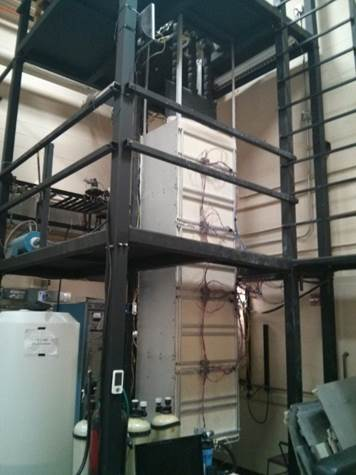
\includegraphics[keepaspectratio,height=0.35\paperheight]{WRCCS_HeaterBox}
            \end{figure}
        \end{column}
    \end{columns}
\end{frame}

\begin{frame}{WRCCS Features}
    \begin{columns}
        \begin{column}{0.71\paperwidth}
        
            \begin{itemize}
                \item $\sim$330 gallon tank, rated for 2 atm
                \item Heater Array
                \begin{itemize}
                    \item maximum $\sim$40 kW radiant power
                    \item<1-> 34 heaters, 17$\times$2 array \only<2>{(old)}
                    \item<2-> 36 heaters, 9$\times$4 array \only<2>{(new)}
                \end{itemize}
                \item Instrumentation
                \begin{itemize}
                    \item Flow meter (total system flow rate)
                    \item Numerous thermocouples
                    \item Differential and absolute pressure
                    \item<2-> Void mesh sensors (new)
                \end{itemize}
            \end{itemize}
        \vfill
            \only<2>{
                \begin{figure}
                    \vskip-3em
                    \hskip14em
                    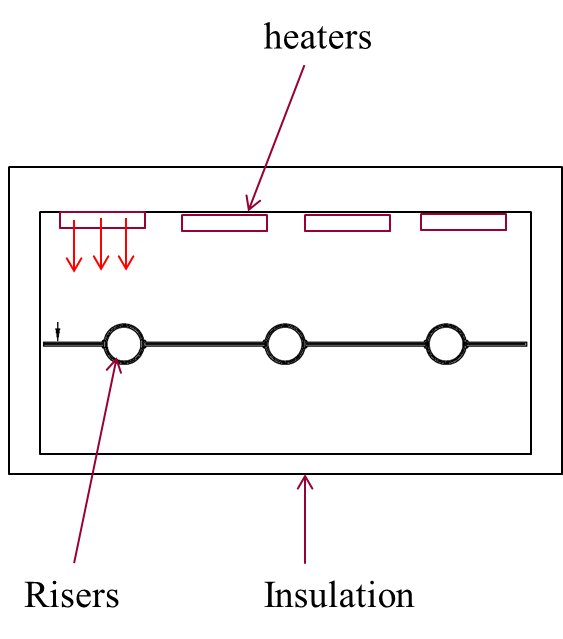
\includegraphics[keepaspectratio,height=0.32\paperheight]{WRCCS_HeaterConfiguration}
                \end{figure}
            }
        \end{column}
        \hfill
        \begin{column}{0.28\paperwidth}
            \begin{figure}
                \centering
                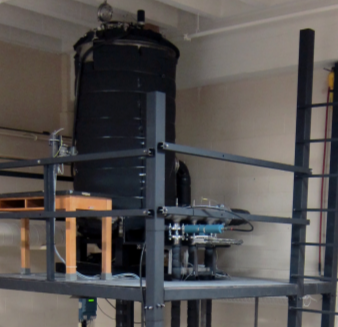
\includegraphics[keepaspectratio,height=0.35\paperheight]{WRCCS_Tank}\\
                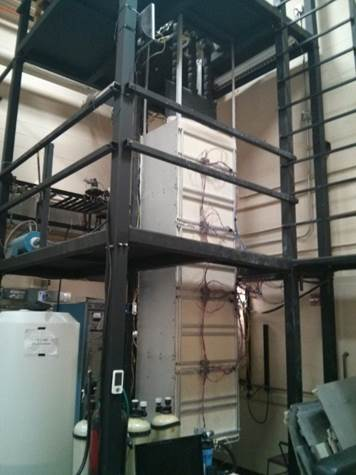
\includegraphics[keepaspectratio,height=0.35\paperheight]{WRCCS_HeaterBox}
            \end{figure}
        \end{column}
    \end{columns}
\end{frame}

\begin{frame}{Boiling Features}
    \begin{description}
        \item[A.] Single-phase heat-up
        \item[B.] Boiling incipience
        \item[C.] Boiling oscillations
        \item[D.] Continuous circulations
        \item[E.] Geysering
    \end{description}
    \begin{figure}%
        \caption{Source:  ``Influences of boil-off on the behavior of a two-phase natural circulation loop'', 2014., \textit{Int. J. of Multiphase Flow}, 60, 135-148.}%
        \vskip-1.2em
        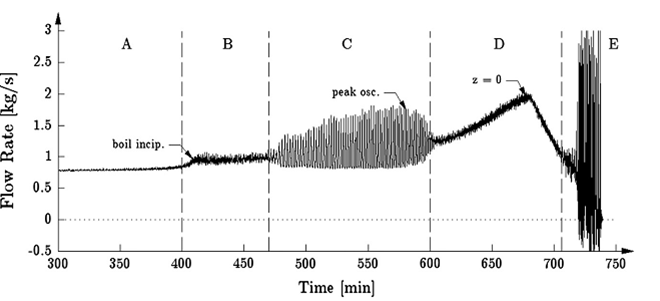
\includegraphics[height=0.425\paperheight]{BoilingRegimes}%
    \end{figure}
\end{frame}

\begin{frame}{Benchmark Test}
    \begin{itemize}
        \item Chose the most mature test for benchmark modeling.
        \item Parameters
        \begin{itemize}
            \item Initial tank fill: 60\%
            \item Power profile: Uniform
            \item No active cooling
        \end{itemize}
    \end{itemize}
    \begin{figure}%
        \caption{Energy balance and mass flow rate of benchmark}%
        \vskip-1em
        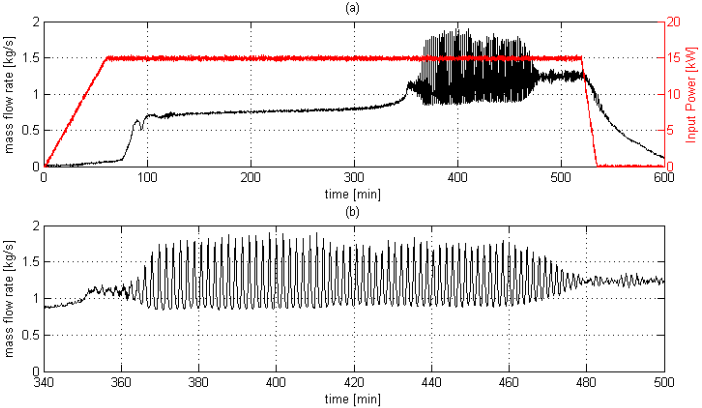
\includegraphics[height=0.46\paperheight]{WRCCS_ExperimentData}%
    \end{figure}
\end{frame}


\section{Modeling}


\begin{frame}{Development}
    \begin{itemize}
        \item Started from simple adiabatic design
        \item Investigated several other variations:
        \begin{itemize}
            \item Tank Nodalization
            \item Heat losses
                \begin{itemize}
                    \item Reduced power
                    \item Heater box losses and air infiltration
                    \item Heat box and network piping losses
                \end{itemize}
            \item Interphase friction
        \end{itemize}
    \end{itemize}
\end{frame}

\begin{frame}{Base Nodalization: Network}
        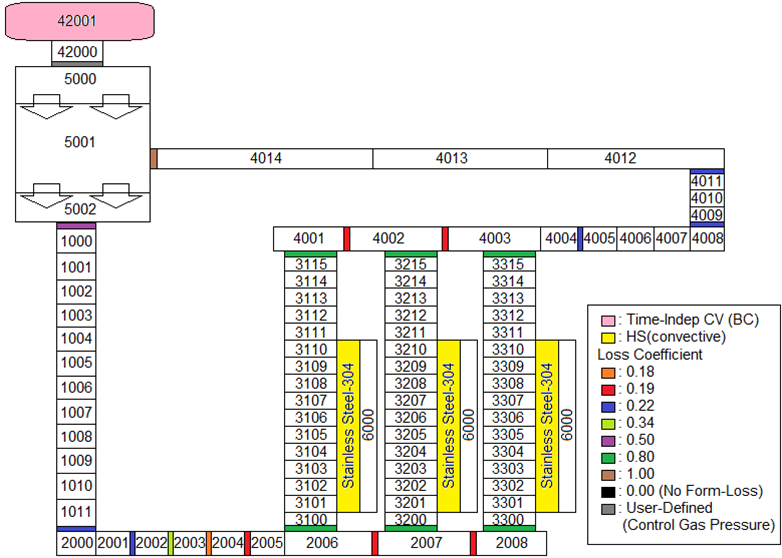
\includegraphics[height=0.75\paperheight]{WRCCS_Nodalization}
        \hfill\textit{\scriptsize Not to-scale}
\end{frame}
\begin{frame}{Base Nodalization: Heater Box}
    \centering
    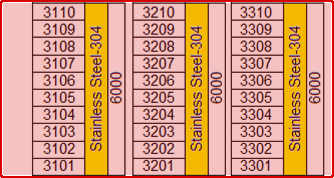
\includegraphics[width=0.3\paperwidth]{WRCCS_Nodalization-HeaterSection}
        
        {\Large $\Downarrow$}
        
    {
    \centering
    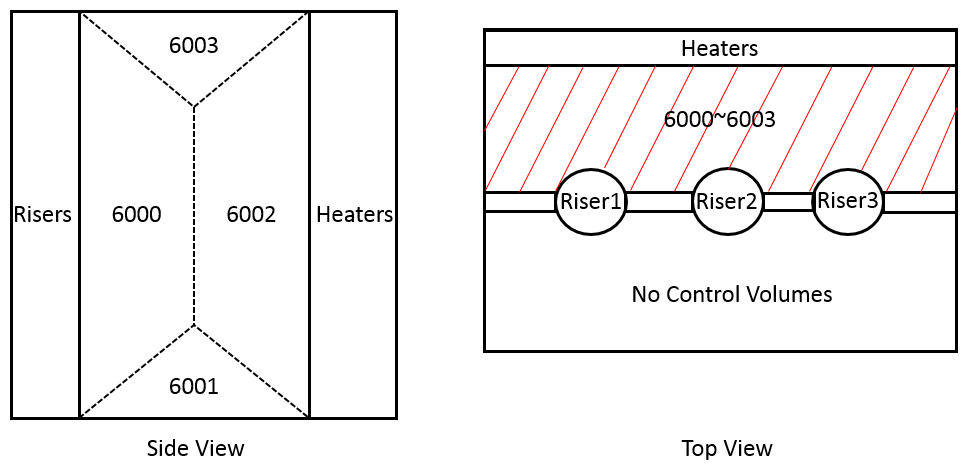
\includegraphics[width=0.65\paperwidth]{WRCCS_CavityNodalization}
    }
        
        \hfill\textit{\scriptsize Not to-scale}
\end{frame}



\subsection{Tank Nodalization}

\begin{frame}{Variations}
    \centering
    \vfill
    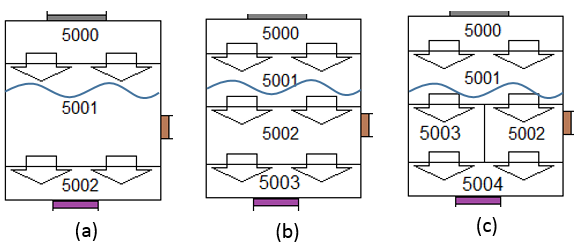
\includegraphics[width=0.75\paperwidth]{TankNodalization}
    \vfill
\end{frame}

\begin{frame}{Comparison}
    \vskip-0.8em
    \centering
    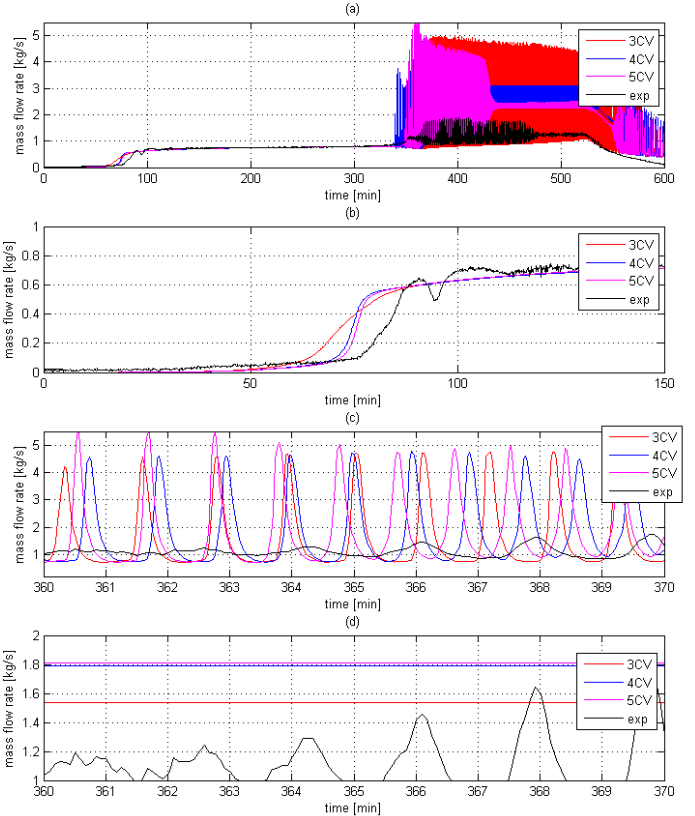
\includegraphics[width=0.69\paperheight]{Comparison_TankNodalization}
\end{frame}




\subsection{Heat Loss Considerations}

\begin{frame}{Adiabatic}
    \centering
    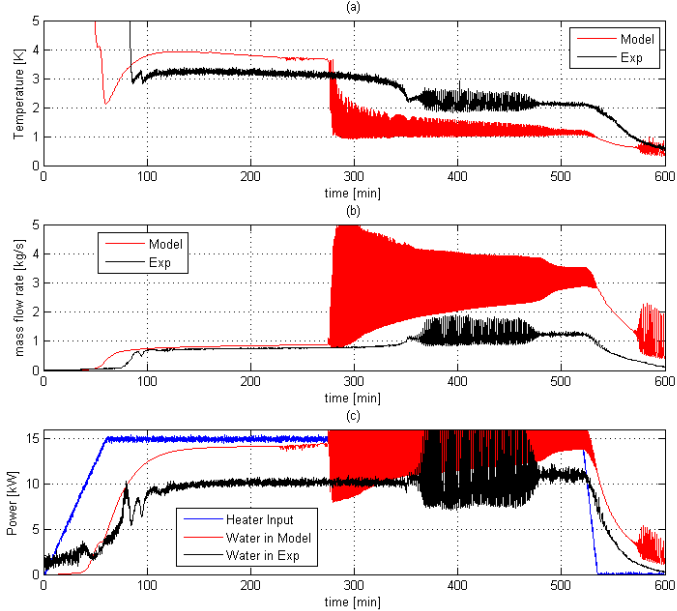
\includegraphics[height=0.77\paperheight]{Comparison_Adiabatic}
\end{frame}
\begin{frame}{Energy losses}
    \begin{itemize}
        \item Experiment is not adiabatic: $\sim4.5$ kW lost in test section
        \item Two different paths were considered
        \begin{itemize}
            \item Reduced power: artificially lower heater power
            \item Heater box loss: add convective losses and air infiltration to heater box
        \end{itemize}
    \end{itemize}
\end{frame}

\begin{frame}{Reduced Power (B)}
    \centering
    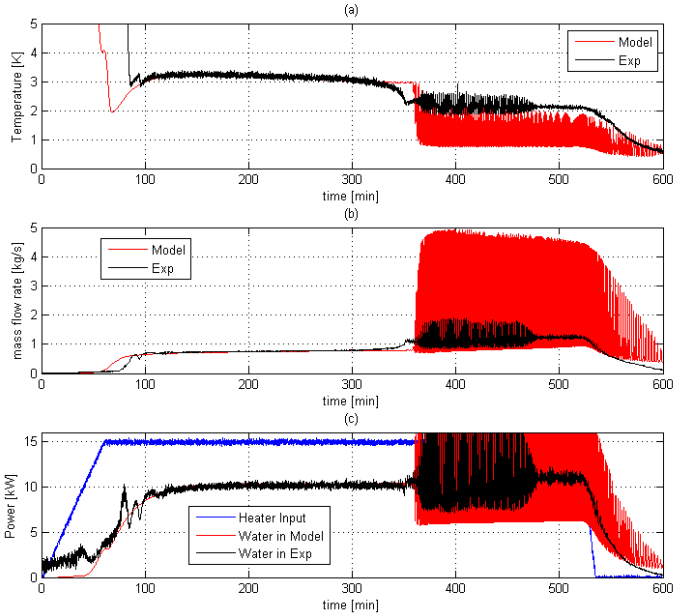
\includegraphics[height=0.77\paperheight]{Comparison_Reduced}
\end{frame}


\begin{frame}{Heater Box Loss  (C)}
    \centering
    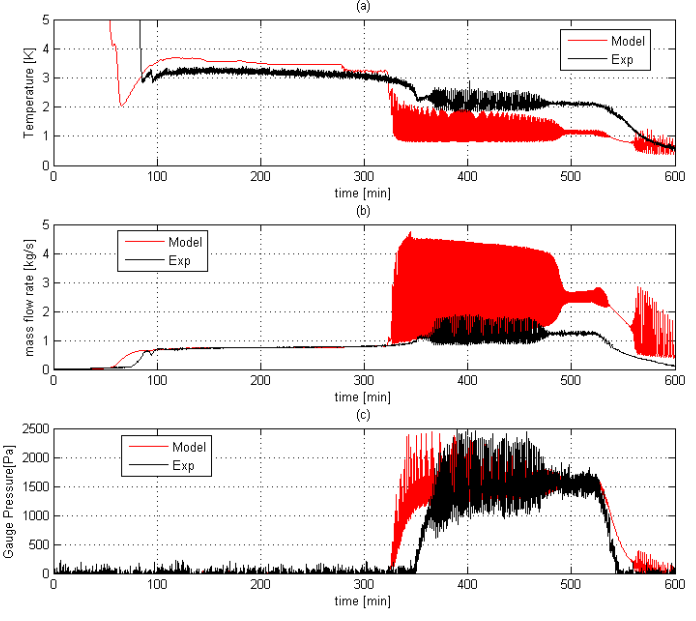
\includegraphics[height=0.77\paperheight]{Comparison_HeaterBoxLoss}
\end{frame}

\begin{frame}{Reduced Power/Convective Losses  (D)}
    \centering
    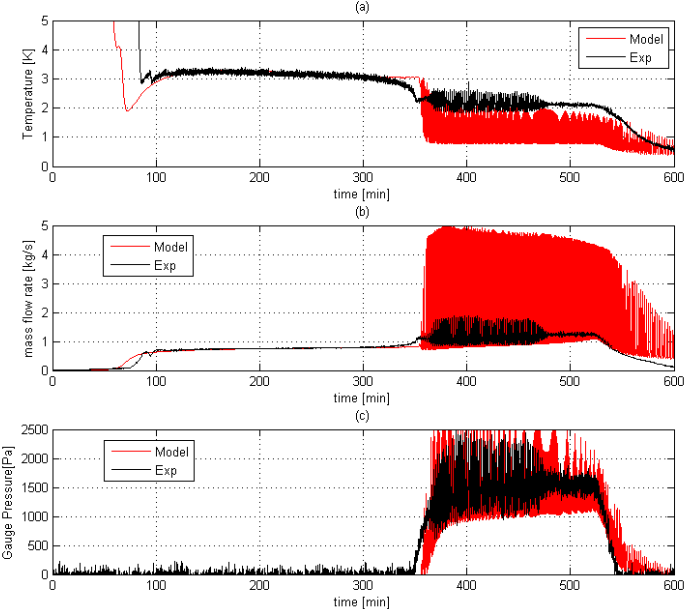
\includegraphics[height=0.77\paperheight]{Comparison_HeaterBoxLoss2}
\end{frame}

\begin{frame}{Piping Loss Comparison}
    \only<1>{
    \begin{itemize}
        \item Additional network piping losses quantified: $\sim2$ kW
        \item Doesn't affect temperature rise
        \item Does affect period and average mass flow rate
    \end{itemize}
    }
    \only<2>{
    \centering
    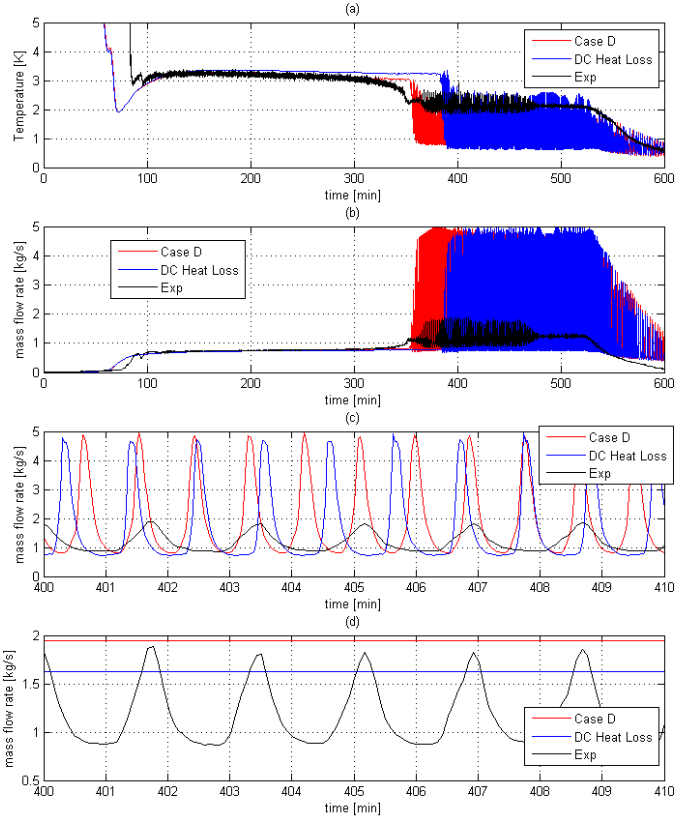
\includegraphics[height=0.77\paperheight]{Comparison_Piping}
    }
\end{frame}


\subsection{Interphase friction}

\begin{frame}{Interphase friction}
    \only<1>{
        MELCOR's interphase friction term was considered to account for period discrepancy.
    }
    \only<2>{
    \centering
    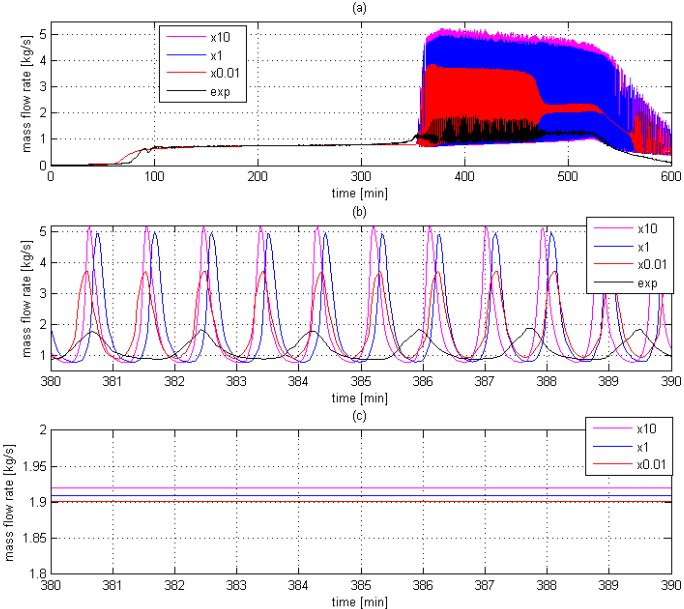
\includegraphics[height=0.77\paperheight]{Comparison_InterphaseFriction}
    }
\end{frame}


\section{Conclusion}

\begin{frame} {Conclusions}
    \begin{itemize}
        \item MELCOR is able to qualitatively model the Heat-Up and Boiling Oscillation regimes
        \item Period/Amplitude discrepancy may imply some two-phase dissipation terms are missing
    \end{itemize}
    
    {
    \centering
    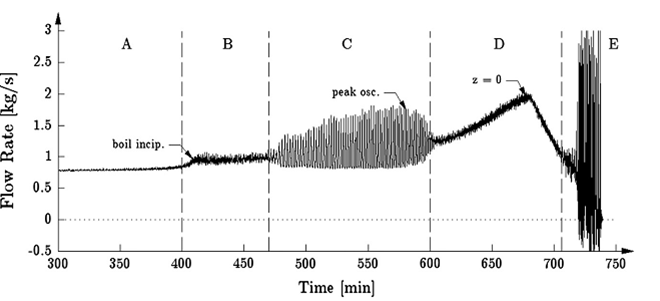
\includegraphics[height=0.27\paperheight]{BoilingRegimes}\vskip0em
    \hfill
    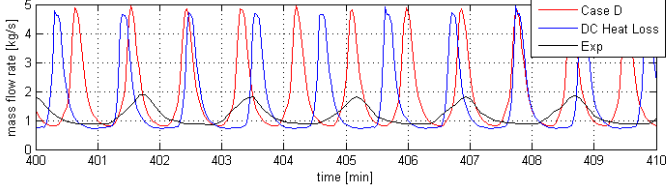
\includegraphics[height=0.27\paperheight]{Comparison_Piping2}%
    \hfill
    }
\end{frame}

\begin{frame} {Current and Future Work}

    \begin{itemize}
        \item Installed Void Mesh Sensors in boiling region of experiment
        \item Use data to infer relationships among system variables (e.g., pressure losses, voiding, and mass flow rate).
    \end{itemize}

        {
        \centering
        \hfill
        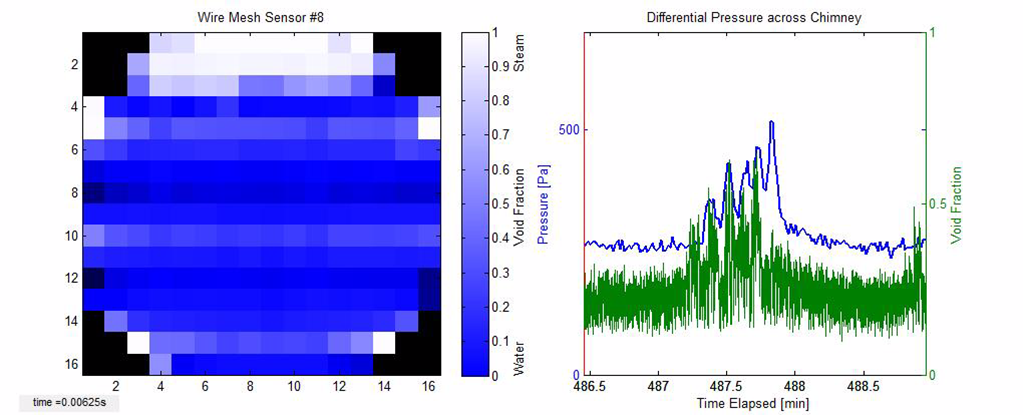
\includegraphics[height=0.50\paperheight]{VoidData_01}%
        \hfill
        }
        
\end{frame}





% ======================================================= %
%                         Questions                       %
% ======================================================= %
\begin{frame}
    \frametitle{~\ }
    \vbox{}\vfill
    \hfill{\Large Questions}\hfill
    \vbox{}\vfill
\end{frame}

\end{document}

